\documentclass[a4paper,notumble]{leaflet}
\usepackage[T1]{fontenc}
\usepackage[utf8]{inputenc}
\usepackage{lmodern}
\usepackage{graphicx}

% PDF properties and links
\usepackage{hyperref}
\hypersetup{
  pdfauthor   = {Sébastien Wilmet},
  pdftitle    = {GNOME Brochure},
  pdfcreator  = {Texlive},
  pdfproducer = {Texlive},
  colorlinks  = false,
  pdfborder   = 0 0 0
}

\title{The GLib/GTK+ Development Platform}
\date{}
\author{}

\begin{document}

\maketitle
\thispagestyle{empty}

GTK+, or the GIMP ToolKit, is a multi-platform toolkit for creating graphical user interfaces. Offering a complete set of widgets, GTK+ is suitable for projects ranging from small one-off tools to complete application suites.

GTK+ is written in C but has been designed from the ground up to support a wide range of languages, not only C/C++. Using GTK+ from languages such as Python and JavaScript (especially in combination with the Glade GUI builder) provides an effective method of application development.

GTK+ is free software and part of the GNU Project. However, the licensing terms for GTK+, the GNU LGPL, allow it to be used by all developers, including those developing proprietary software, without any license fees or royalties.

GTK+ has been created in 1996 for the GIMP --- the GNU Image Manipulation Program --- but has quickly become a general-purpose library used by a large number of applications including the GNU project's GNOME desktop.

\begin{center}
  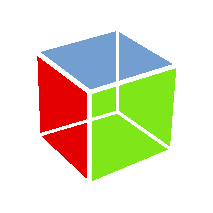
\includegraphics[width=3cm]{images/gtk-logo.pdf}
  \hspace{1cm}
  
\includegraphics[width=2cm]{images/gnome-logo.pdf}
\end{center}

\pagebreak

\section{Architecture Overview}

Over time GTK+ has been built up to be based on other libraries, also developed by the GTK+ team:
\begin{itemize}
  \item \textbf{GLib}, a low-level core library that forms the basis of GTK+. It provides data structure handling for C, portability wrappers and interfaces for such run-time functionality as an event loop, threads, dynamic loading, an object system (GObject) and high-level input/output APIs (GIO).

  \item \textbf{Pango}, a library for layout and rendering of text with an emphasis on internationalization. It forms the core of text and font handling for GTK+.

  \item \textbf{Cairo}, a library for 2D graphics with support for multiple output devices (including the X Window System, Win32) while producing a consistent output on all media while taking advantage of display hardware acceleration when available.

  \item \textbf{ATK}, a library for a set of interfaces providing accessibility. By supporting the ATK interfaces, an application or toolkit can be used with tools such as screen readers, magnifiers, and alternative input devices.

  \item \textbf{GDK}, or the GIMP Drawing Kit, is the abstraction layer that allows GTK+ to support multiple windowing systems. GDK provides backends for X11, Windows, Mac OS X, Wayland, Mir, and a web browser.
\end{itemize}

\vspace{1cm}
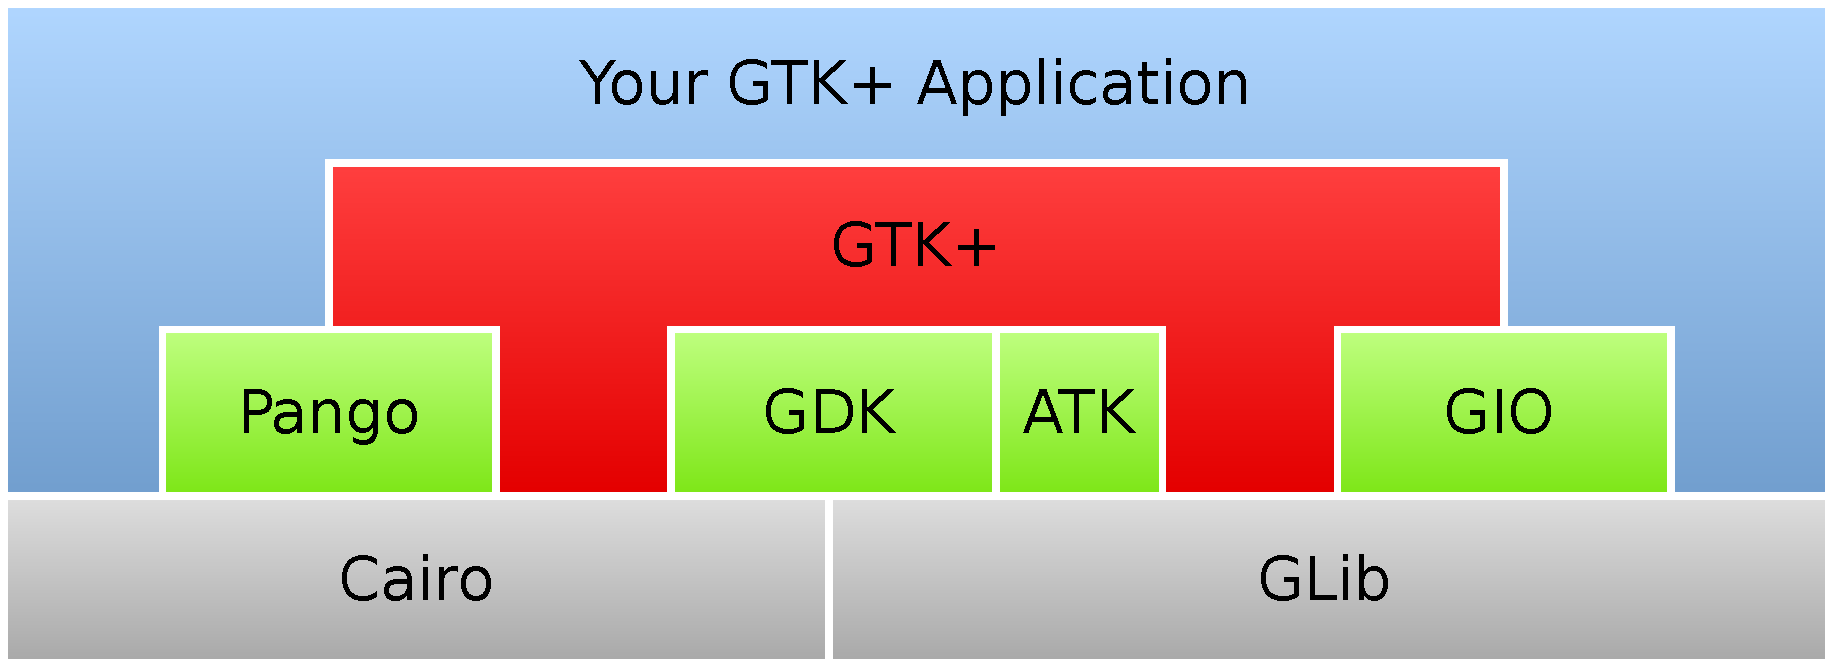
\includegraphics[width=\textwidth]{images/architecture.pdf}

\section{GLib -- the Core Library}

\section{GObject -- an Object System}

\section{GIO -- Input/Output on Steroids}

\section{The GTK+ Widget Toolkit}

\end{document}
